\documentclass[a4paper,10pt]{article}
\usepackage[dvips]{color,graphicx}
\usepackage[dvips, bookmarks, colorlinks=false]{hyperref}
\addtolength{\textwidth}{3.5cm}
\addtolength{\hoffset}{-2cm}

%opening
\title{Math650 Homework 6}
\author{Yu Huang}
\date{}

\begin{document}

\maketitle

\begin{abstract}

\end{abstract}

\section{Introduction}
Using Linear Regression technique to study the relationship between Wine Consumption and Heart Disease.

\section{Materials and Methods}
Chapter 8 Problem 23. Methods are various statistics functions of software R (code appended~\ref{appendix}).

\section{Results}
\subsection{Data not logged}
Directly applying linear model over the original data, we get following summary result.
\begin{verbatim}
Residuals:
    Min      1Q  Median      3Q     Max
-2.0683 -1.3616 -0.2138  1.4897  2.8406

Coefficients:
            Estimate Std. Error t value Pr(>|t|)
(Intercept)  7.68655    0.47332  16.240 2.31e-11 ***
WINE        -0.07608    0.01700  -4.475 0.000383 ***
---
Signif. codes:  0 '***' 0.001 '**' 0.01 '*' 0.05 '.' 0.1 ' ' 1

Residual standard error: 1.619 on 16 degrees of freedom
Multiple R-Squared: 0.5559,     Adjusted R-squared: 0.5281
F-statistic: 20.03 on 1 and 16 DF,  p-value: 0.0003828
\end{verbatim}

All the associated figures are in Figure~\ref{f1}. The \emph{Residuals vs Fitted}, \emph{Scale-Location} and scatterplot(\emph{MORTALITY vs WINE} all shows data is clottered into one end in terms of X-axis. \emph{Normal Q-Q} shows the distribution of residuals are long-tailed. \emph{Residuals vs Leverage} shows some points with high leverage have high cook's distance, which suggests these points have high influence but low prediction power. While doing leave-one-out prediction for these points, the value deviated a lot from the true value.

\begin{figure}[p]
\includegraphics[angle=-90, width=1\textwidth]{figures/hw6_fig1.eps}
\caption{WINE is not logged}\label{f1}
\end{figure}

\subsection{Data logged}
After the WINE data(X-axis) is logged, the data looks better.
\begin{verbatim}
Residuals:
    Min      1Q  Median      3Q     Max
-2.2559 -1.0849 -0.1914  0.7326  2.5687

Coefficients:
            Estimate Std. Error t value Pr(>|t|)
(Intercept)  10.2795     0.8316  12.360 1.34e-09 ***
WINE         -1.7712     0.3468  -5.108 0.000105 ***
---
Signif. codes:  0 '***' 0.001 '**' 0.01 '*' 0.05 '.' 0.1 ' ' 1

Residual standard error: 1.498 on 16 degrees of freedom
Multiple R-Squared: 0.6199,     Adjusted R-squared: 0.5961
F-statistic: 26.09 on 1 and 16 DF,  p-value: 0.0001054
\end{verbatim}
The p-values for coefficient of WINE, F-statistic are more significant. R-Squared shows an increase(More variation can be explained by the model). All the associated figures~\ref{f2} also shows this improvement. 


\begin{figure}[p]
\includegraphics[angle=-90, width=1\textwidth]{figures/hw6_fig2.eps}
\caption{WINE is logged}\label{f2}
\end{figure}

\section{Conclusion and Discussion}
Based on the data, there's association between MORTALITY and WINE consumption. Shortly, the more wine consumed, the lower mortality(heart disease) rate.

One thing to notice is that we are working on group means(both MORTALITY and WINE are means over population in each country.), which is the so-called ecological correlation. Ecological correlation tends to overstate the strength of association. Be careful when extrapolating this conclusion to the individuals in each country, which is not the level we are working on(we are working on country-level).

\section{Appendix}
\label{appendix}
\begin{verbatim}
linear_model_func = function(data, output_fname)
{
	result = lm(MORTALITY ~ WINE, data)
	print(summary(result))
	#hist(resid(result))
	#qqnorm(resid(result))
	postscript(output_fname)
	opar <- par(mfrow = c(3,2), oma = c(0, 0, 1.1, 0))
	#'oma' A vector of the form 'c(bottom, left, top, right)' giving the size of the outer margins in lines of text.
	plot(result)
	
	#par(opar)
	#dev.off()
	#postscript(output_fname)
	#opar <- par(mfrow = c(1,2), oma = c(0, 0, 1.1, 0))
	
	#plot(fitted(result), resid(result), main='fitted value vs residual')
	plot(data$WINE, data$MORTALITY, main='MORTALITY vs WINE', xlab='WINE', ylab='MORTALITY')
	abline(result, col=4)
	par(opar)
	dev.off()
}

data = read.csv("/usr/local/doc/statistical_sleuth/ASCII/ex0823.csv")
output_fname = '~/script/test/math650/figures/hw6_fig1.eps'
linear_model_func(data, output_fname)
new_data = data
new_data$WINE = log(new_data$WINE)
output_fname2 = '~/script/test/math650/figures/hw6_fig2.eps'
linear_model_func(new_data, output_fname2)
\end{verbatim}

\end{document}
